\documentclass[12pt,letterpaper]{article}

\usepackage[utf8]{inputenc}
\usepackage[T1]{fontenc}
\usepackage{amsmath}
\usepackage{amsfonts}
\usepackage{amssymb}
\usepackage{amsthm}
\usepackage[left=2cm,right=2cm,top=2cm,bottom=2cm,headheight=22pt]{geometry}
\usepackage{fancyhdr}
\usepackage{setspace}
\usepackage{lastpage}
\usepackage{graphicx}
\usepackage{caption}
\usepackage{subcaption}
\usepackage{paralist}
\usepackage{tikz}

\theoremstyle{definition}
\newtheorem{question}{Question}
\newtheorem{example}{Example}
\newtheorem{exercise}[question]{Exercise}
\newtheorem*{challenge}{Challenge}
\newtheorem*{theorem}{Theorem}
\newtheorem*{problem}{Problem}

\begin{document}

%Paramètres de mise en forme des paragraphes selon les normes françaises
\setlength{\parskip}{1ex plus 0.5ex minus 0.2ex}
\setlength{\parindent}{0pt}

%Paramètres relatifs aux en-têtes et pieds de page.
\pagestyle{fancy}
\lhead{Theron J Hitchman}
\chead{\Large Reading and Guided Practice \#6}
\rhead{Spring 2014}
\lfoot{\emph{Math and Decision Making}}
\cfoot{}
\rfoot{\emph{\thepage\ of \pageref{LastPage}}}

\section*{Introduction}
In this reading, you will learn about Reidemeister moves and their significance for knot theory.

\section*{Goals}
At the end of this assignment, a student should be able to:
\begin{compactitem}
\item Identify and use the three Reidemeister moves when discussing knot equivalence.
\item Show two knots are equivalent by ambient isotopy by exhibiting a sequence of Reidemester moves.
\end{compactitem}
A student might also be able to:
\begin{compactitem}
\item Solve a challenging problem using Reidemeister moves.
\end{compactitem}

\section*{Reading and Questions for Topology Meeting 7}

\subsection*{Context and History for the Reidemeister moves}
We have seen that the natural way to view two knots as equivalent is the notion of \emph{ambient isotopy}.
We have also played around enough to see that this is very tricky.
There is no way to collect ``all of the ambient isotopies possible'' and make sure we have checked them---there are simply too many strange things one can do.

Fortunately, there is a way around this, first described by J.~W.~Alexander and G.~B.~Briggs \cite{AB} and independently by H.~Reidemeister \cite{R}.
There are some simple manipulations one can do to a planar projection of a knot, called \emph{Reidemeister moves}.
They are important because of the following result, which was proved in the 1920's.
\begin{theorem}
Suppose that one is given two planar projections of knots.
Then these knots are equivalent by ambient isotopy if and only if there is a finite sequence of \emph{Reidemeister moves} which turns one planar projection into the other.
\end{theorem}

This is exceedingly good news!
You don't have to check ``everything,'' just sequences of these special moves on knots.

The general problem for comparing two knots is still unsolved, but significant work has been done on the ``unknotting problem.''
\begin{problem}
When and how can you tell if a given planar projection of a knot actually represents the unknot?
\end{problem}
It is known that there is an algorithm for deciding this question, but the paper describing it  (by Haken \cite{Haken}) is well over 100 pages long.
In principle, this means someone could program a computer to check if a given diagram was an unknot or not.
[I do not believe anyone has done this.]
One problem that could occur is that even if such a computer program could be designed, it might take an unreasonably long time to compute and give you a response.
How long might it take?
In 1998, Joel Hass and Jeffrey Lagarias proved that it might be long, but not \emph{too} long.
Specifically, they showed this:
\begin{theorem}
For any planar projection of the unknot having $n$ crossings, there is a sequence of Reidemeister moves which transforms the projection into a regular circle and takes no more than $2^{10^{11}n}$ moves.
\end{theorem}

%That is a big number.
%In particular, if $n=6$, then $2^{10^{11}\cdot 6}$ is big enough to break my best computer algebra system.
%Fortunately, computers are getting faster and faster.


\subsection*{The Reidemeister Moves}

So what are the Reidemeister moves?
Each move describes a way in which you can change some small bit of information about a crossing in your planar projection without changing the essential qualities of the knot.
There are three types of moves, and they are easier to see than to describe.

Reidemeister Move 1 either twists or untwists a simple loop in a single strand.
Note this changes the number of crossings by one: an increase of one crossing if adding a twist, a decrease of one crossing if removing a twist.

\begin{figure}[h]
    \centering
    \begin{subfigure}{.3\textwidth}
        \centering
        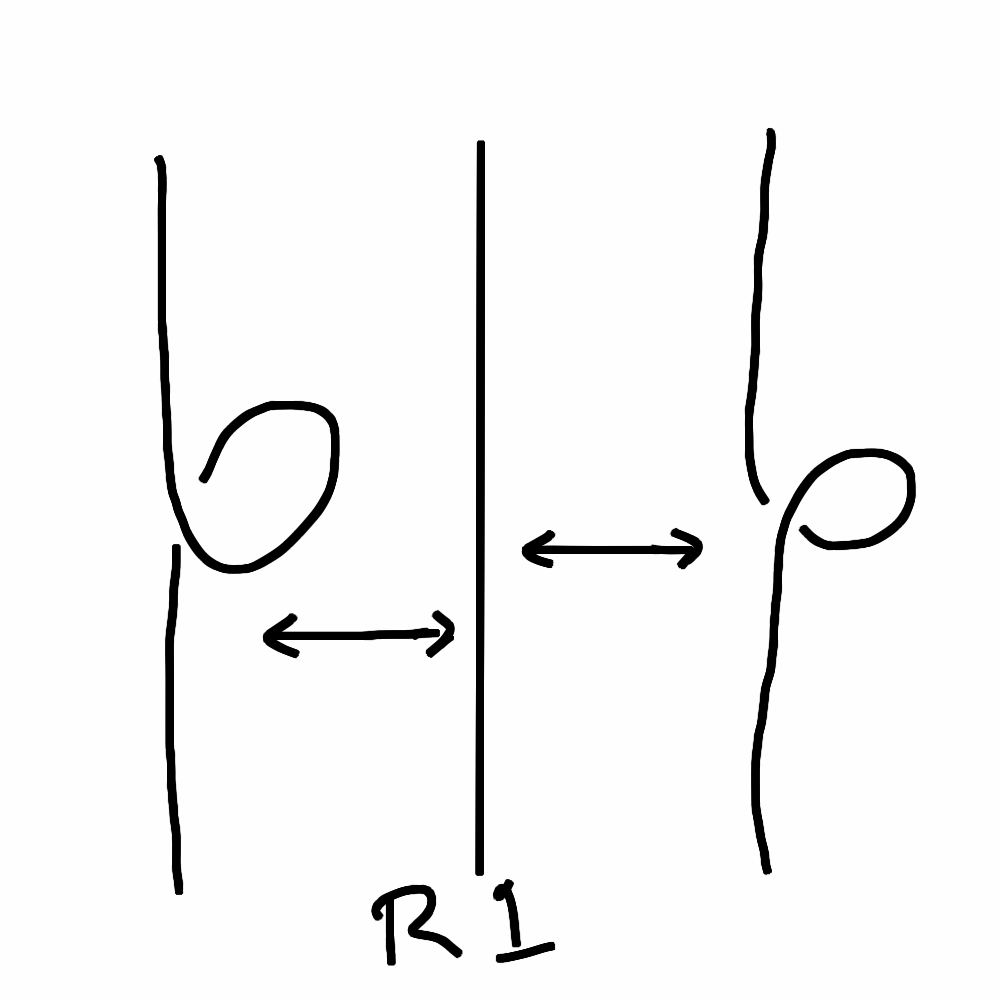
\includegraphics[width=\textwidth]{knotpics/r1.png}
        \caption{Type 1 Reidemesiter Moves}
    \end{subfigure}
    \hspace{1in}
    \begin{subfigure}{.3\textwidth}
        \centering
        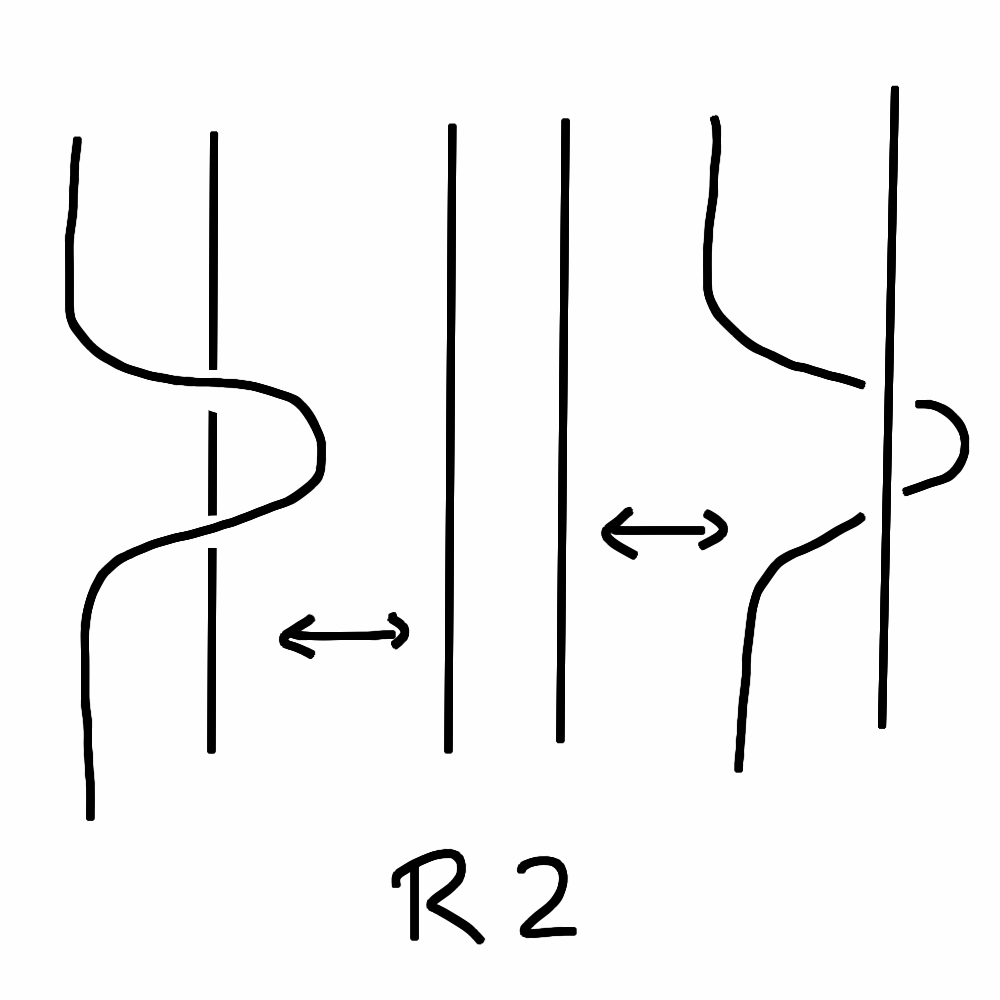
\includegraphics[width=\textwidth]{knotpics/r2.png}
        \caption{Type 2 Reidemesiter Moves}
    \end{subfigure}
    \caption{Reidemeister Moves of type 1 and 2}
\end{figure}

Reidemeister Move 2 either creates or removes a pair of consecutive overcrossings (or undercrossings) of one strand across another.
Note that this changes the number of crossings by 2, up or down.

Type 3 Reidemeister moves do not change the number of crossings in the planar projection, as all we do is move one strand completely across a crossing of two other strands.

\begin{figure}[h]
    \centering
    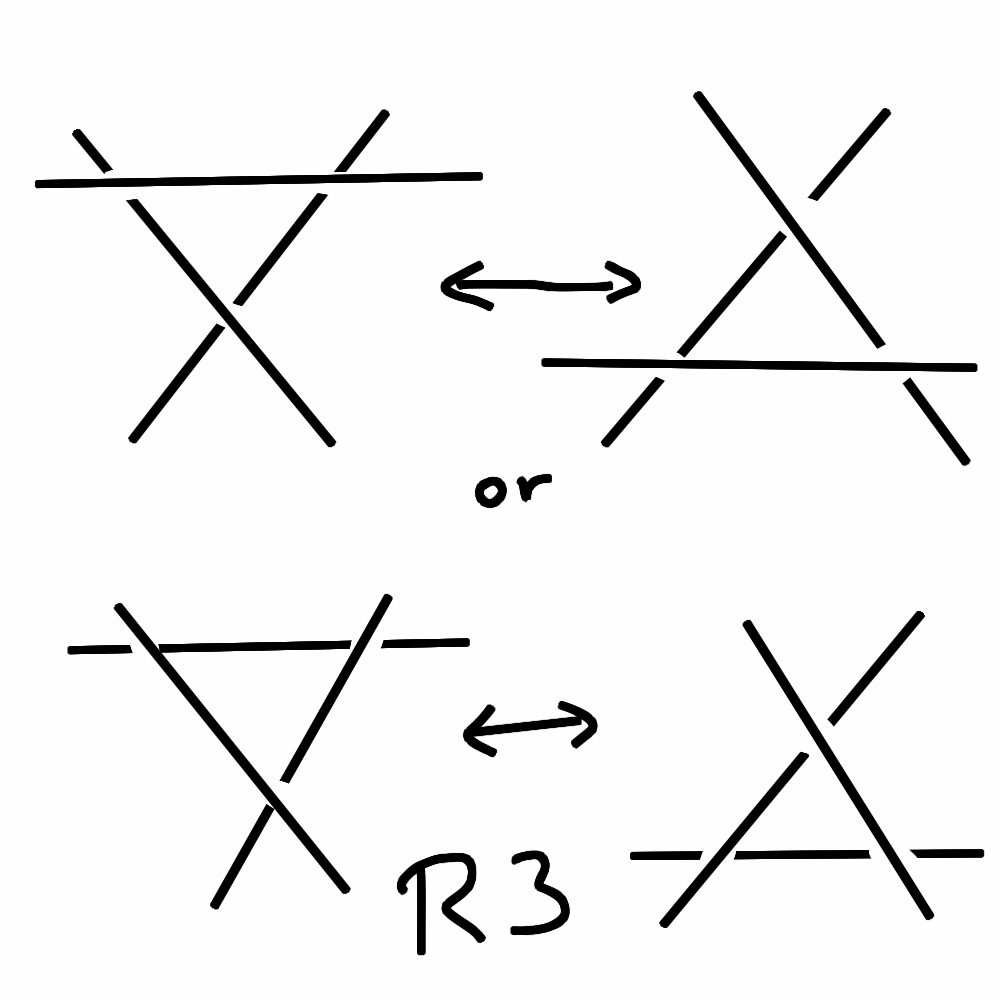
\includegraphics[width=.3\textwidth]{knotpics/r3.png}
    \caption{Type 3 Reidemeister Moves}
\end{figure}



\subsubsection*{Examples and Practice}

Let us see how to handle some examples of equivalence of planar projections using Reidemeister moves and isotopy.

\begin{example}
A simple trefoil with a cheap disguise.
We just untwist.
\end{example}

\begin{figure}[h]
    \centering
    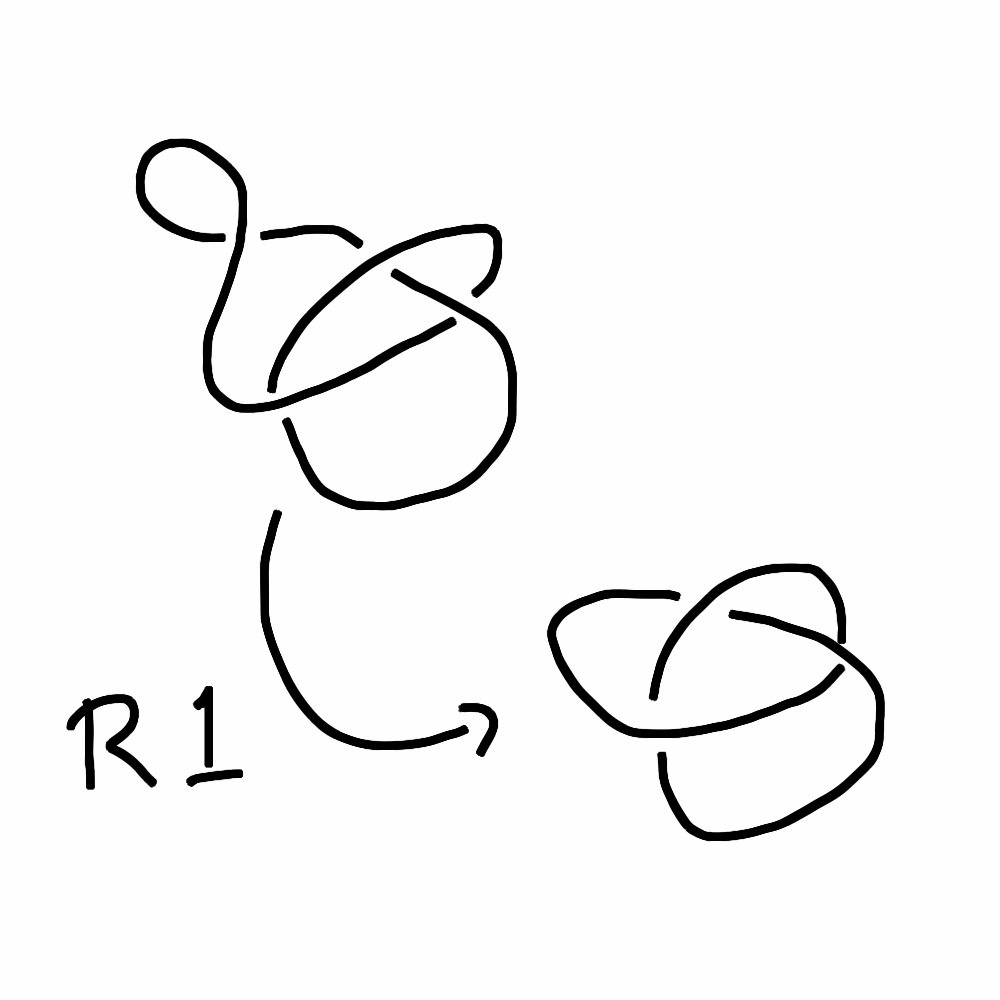
\includegraphics[width=.3\textwidth]{knotpics/trefoil-bad-disguise.png}
    \caption{Trefoil with glasses and a fake mustache.}
\end{figure}

\begin{example}
A trefoil with a better disguise.
Here we bring the far right strand ``under the rest of the diagram'' and then untwist.
\end{example}

\begin{figure}[h]
    \centering
    \begin{subfigure}{.4\textwidth}
        \centering
        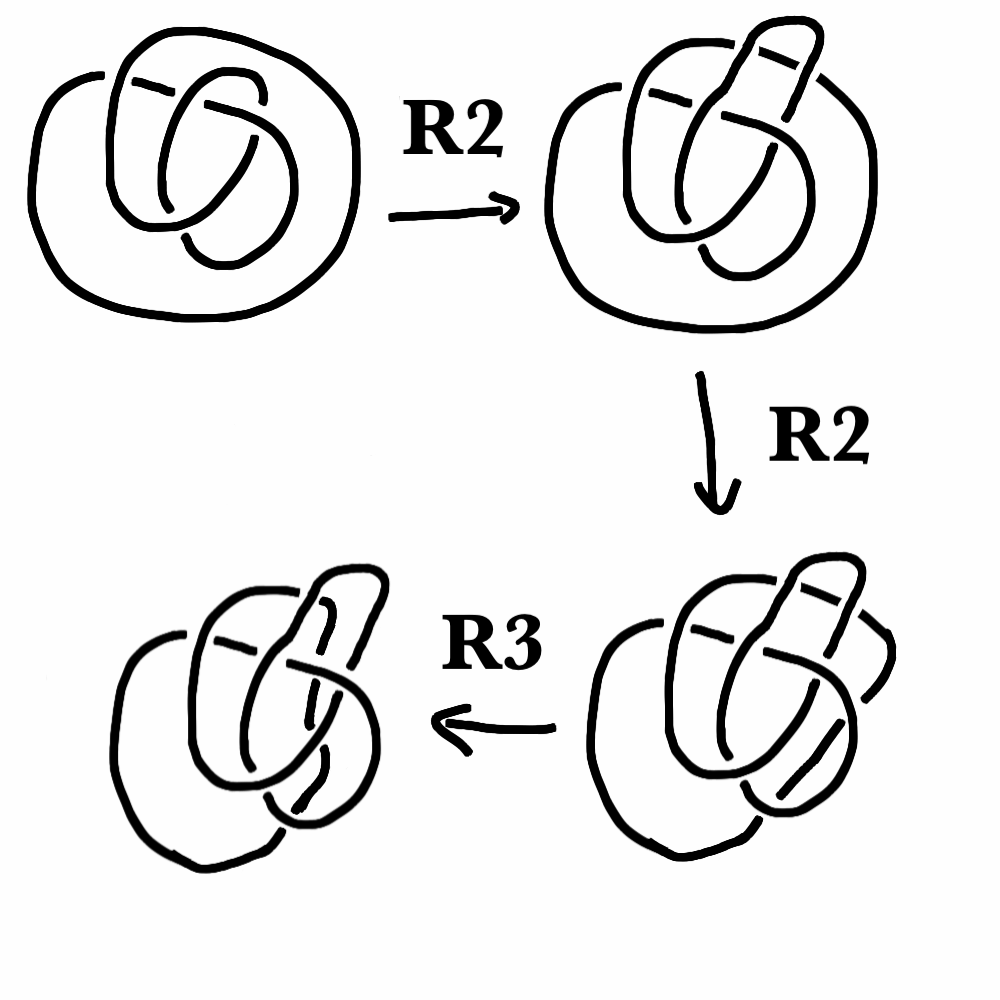
\includegraphics[width=\textwidth]{knotpics/trefoil-better1.png}
        \caption{The first few RMs.}
    \end{subfigure}
    \hspace{2cm}
    \begin{subfigure}{.4\textwidth}
        \centering
        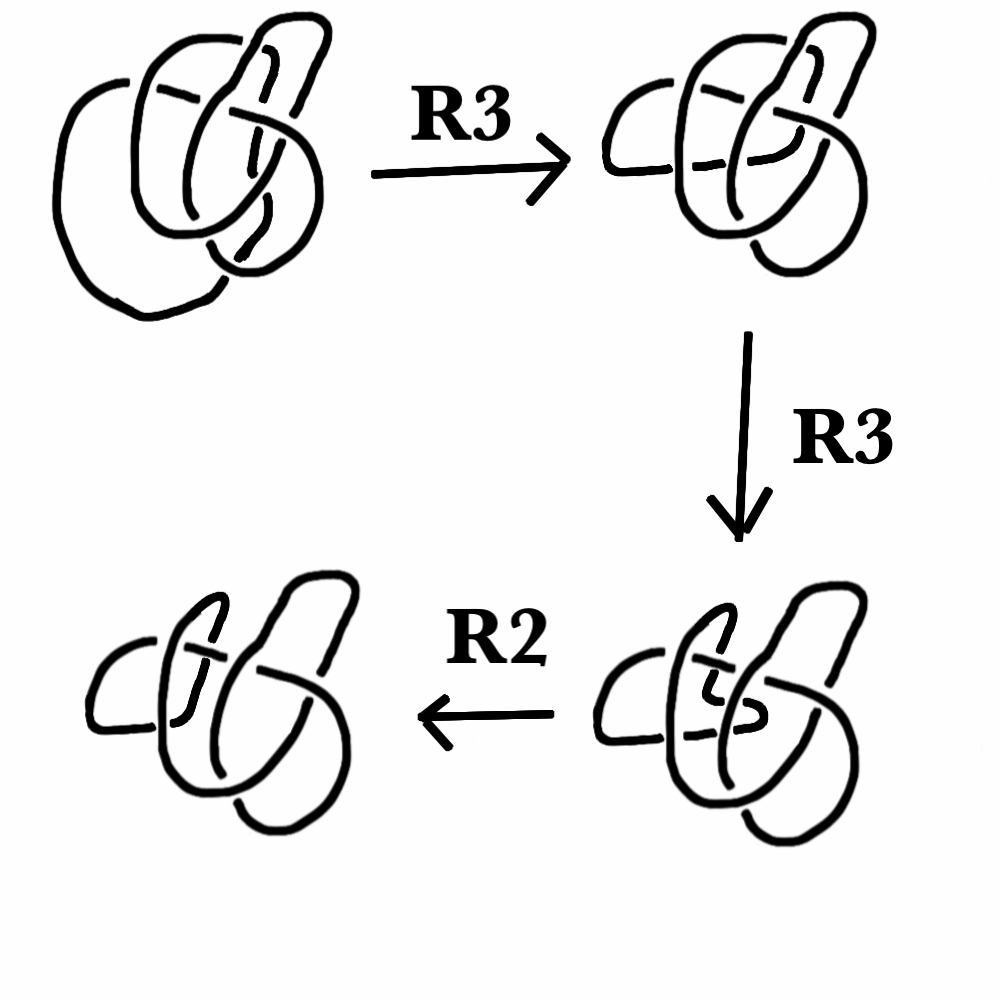
\includegraphics[width=\textwidth]{knotpics/trefoil-better2.png}
        \caption{More RMs, the middle stages.}
     \end{subfigure}
     \caption{Applying Reidemeister Moves to an odd projection of a Trefoil.}
\end{figure}
Note that the upper left projection in Figure 4b is the same as the lower left in Figure 4a.
We are getting closer.
The final few diagrams look like this:

\clearpage

\begin{figure}[h]
    \centering
    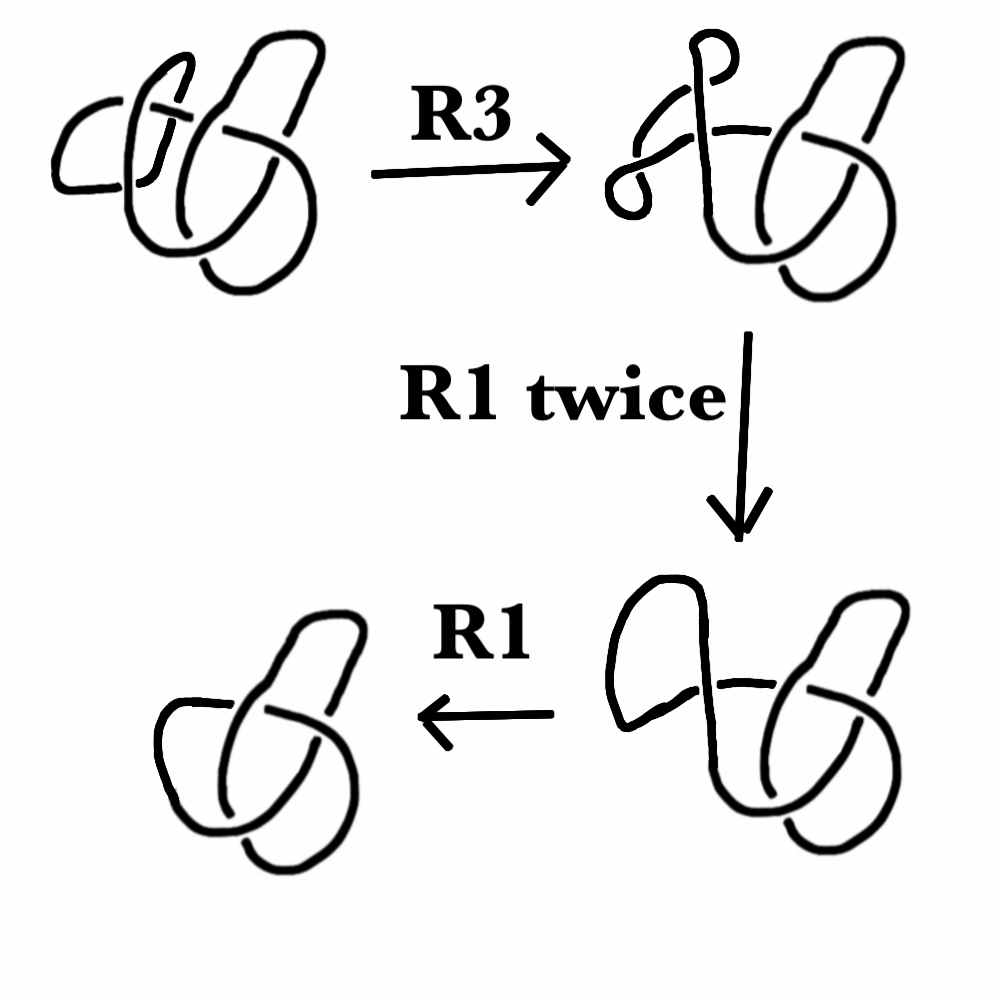
\includegraphics[width=.5\textwidth]{knotpics/trefoil-better3.png}
    \caption{Finally!}
\end{figure}

Well, that was exciting.
Now we should practice.

\begin{exercise} Consider the two planar projections of the figure eight knot below.
These are equivalent by a process similar to our second example above.
Use a sequence of Reidemeister moves to demonstrate that these knots are equivalent.
Draw each intermediate knot, and label the sequence of Reidemeister moves you use as you go.
\end{exercise}

\begin{figure}[h]
    \centering
    \begin{subfigure}{.3\textwidth}
        \centering
        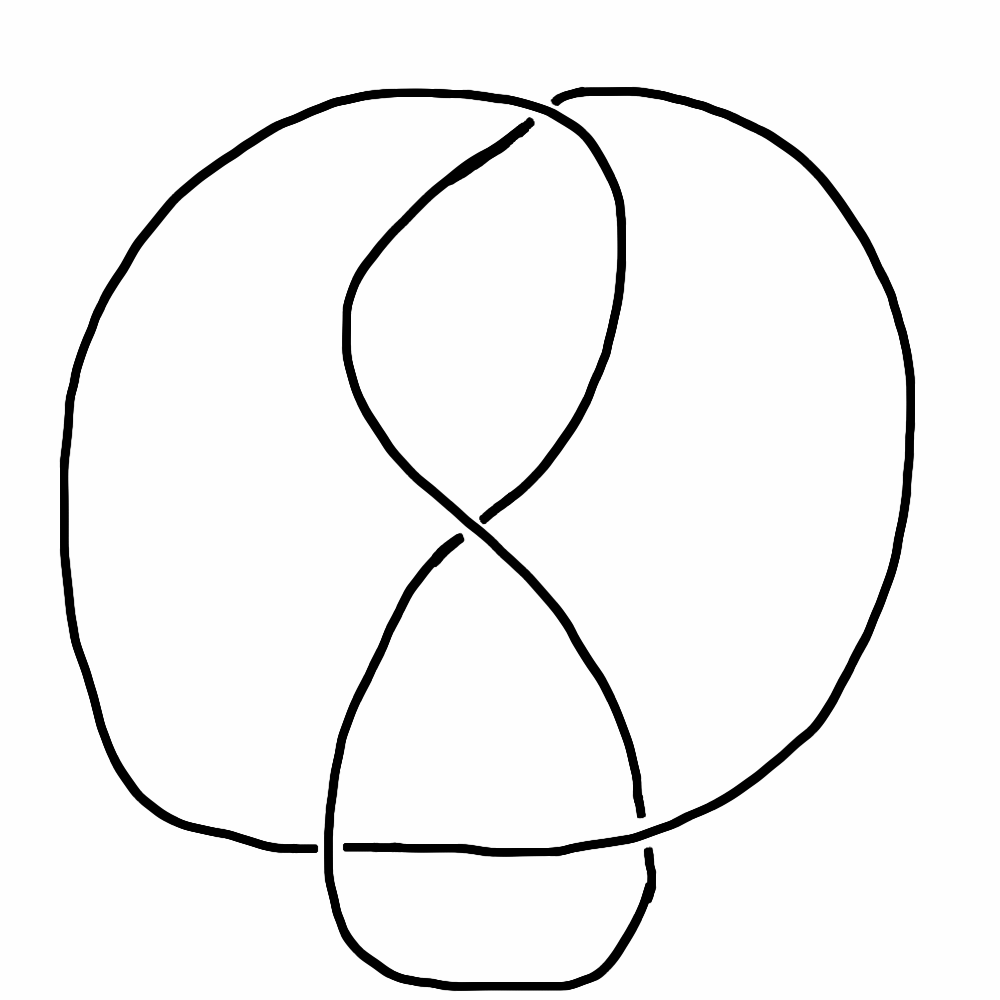
\includegraphics[width=\textwidth]{knotpics/9SeptQ3a.png}
        \caption{The figure eight knot.}
    \end{subfigure}
    \hspace{2cm}
    \begin{subfigure}{.3\textwidth}
        \centering
        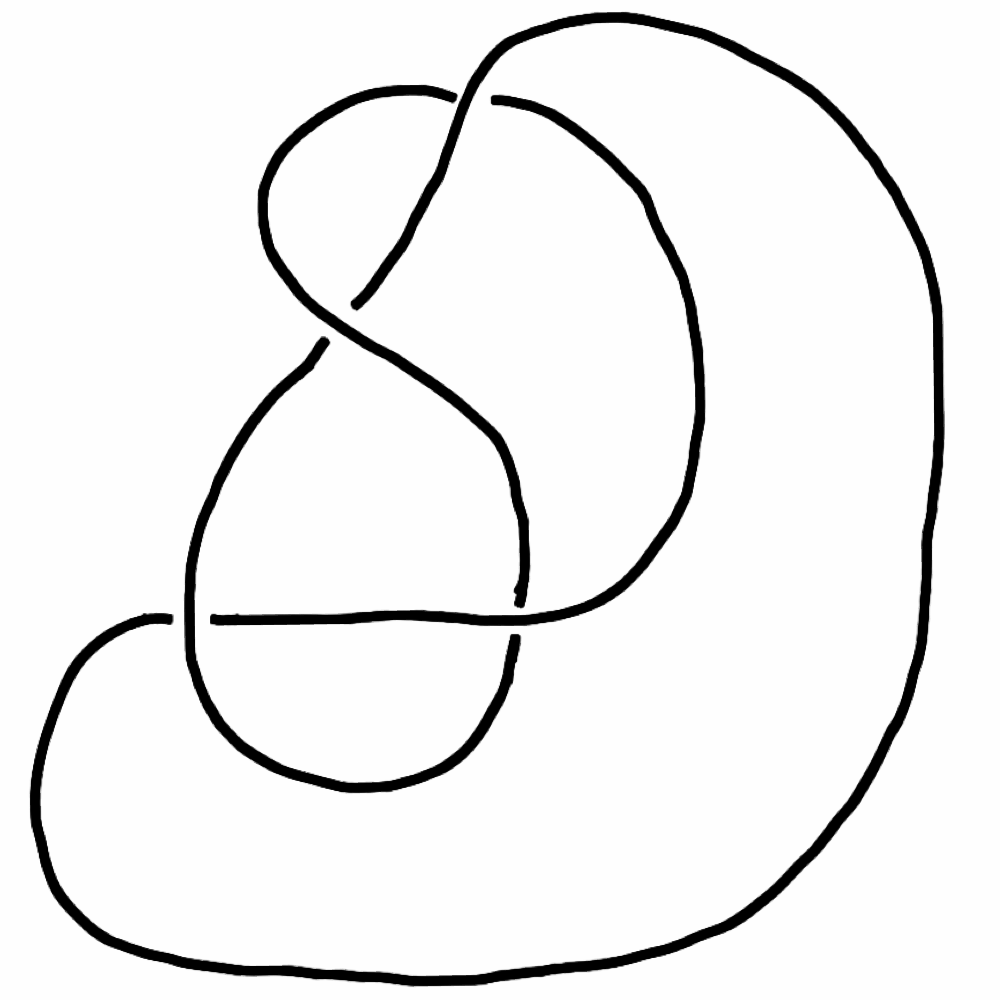
\includegraphics[width=\textwidth]{knotpics/9SeptQ3b.png}
        \caption{Another figure eight knot.}
    \end{subfigure}
    \caption{Show these are the same by Reidemeister moves.}
\end{figure}

\clearpage

\begin{exercise} Consider the two planar projections of the knot below.
Use a sequence of Reidemeister moves to demonstrate that these knots are equivalent.
Draw each intermediate knot, and label the sequence of Reidemeister moves you use as you go.
\end{exercise}


\begin{figure}[h]
    \centering
    \begin{subfigure}{.4\textwidth}
        \centering
        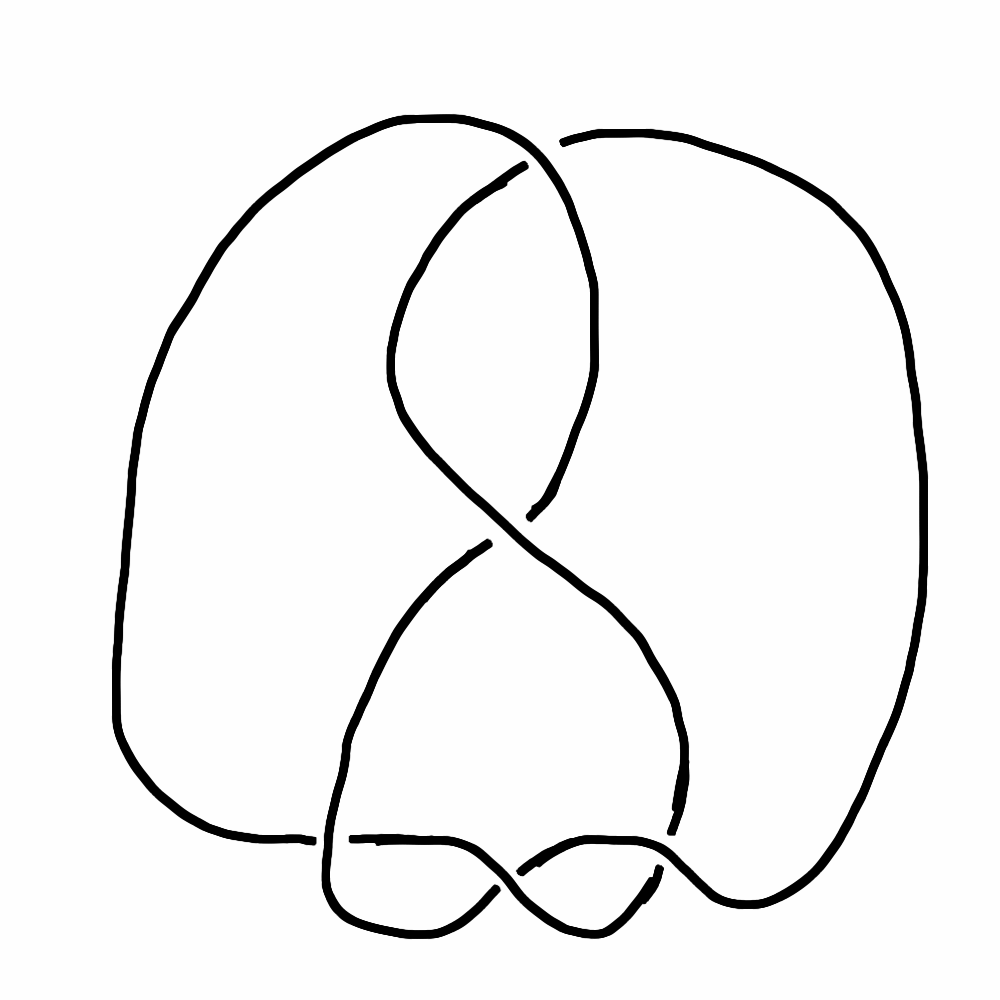
\includegraphics[width=\textwidth]{knotpics/exercise2-1.png}
        \caption{A nice knot.}
    \end{subfigure}
    \hspace{2cm}
    \begin{subfigure}{.4\textwidth}
        \centering
        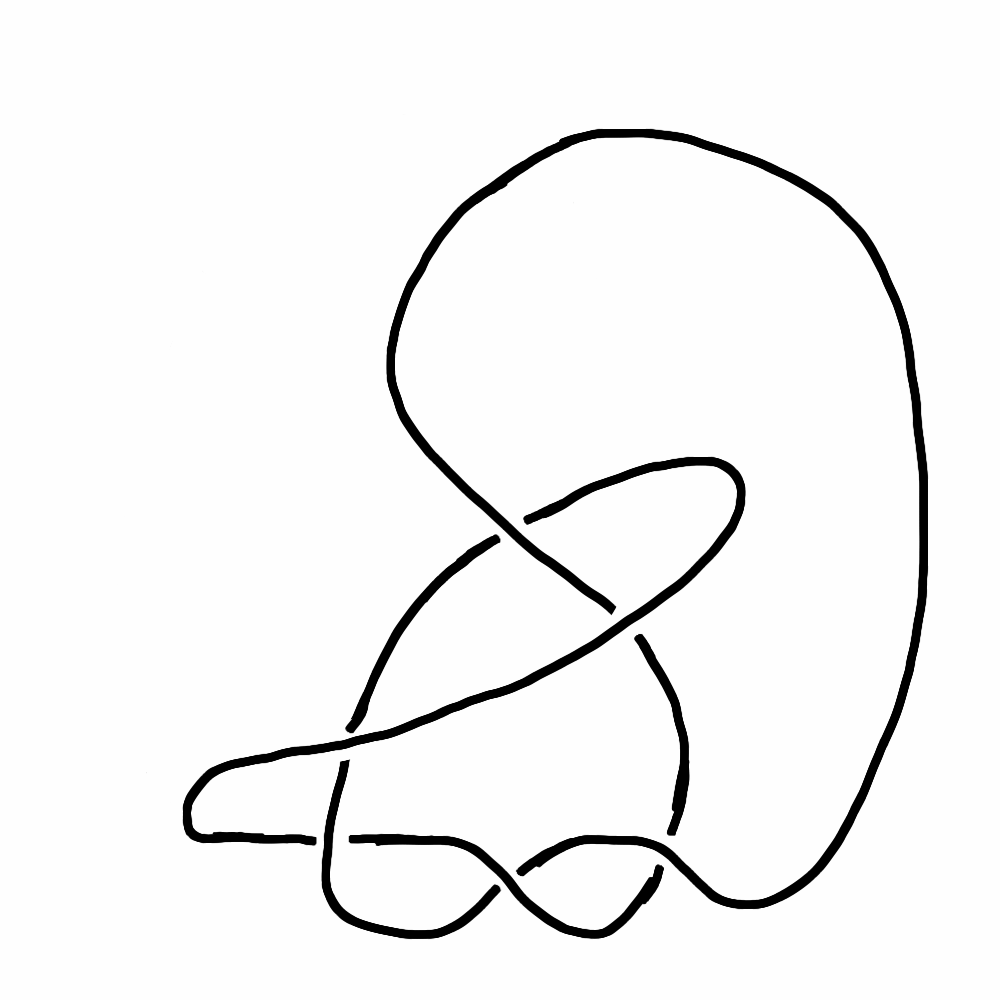
\includegraphics[width=\textwidth]{knotpics/exercise2-2.png}
        \caption{Another nice knot.}
    \end{subfigure}
    \caption{Show these are the same by Reidemeister moves.}
\end{figure}






\begin{challenge}
The following knot is due to Goeritz \cite{G}. It is known to be a projection of the unknot and it has 9 crossings.
Use a sequence of Reidemeister moves to show that this is the unknot.
Somewhere along the line, your diagram should have more than 9 crossings.
\end{challenge}

\begin{figure}[h]
    \centering
    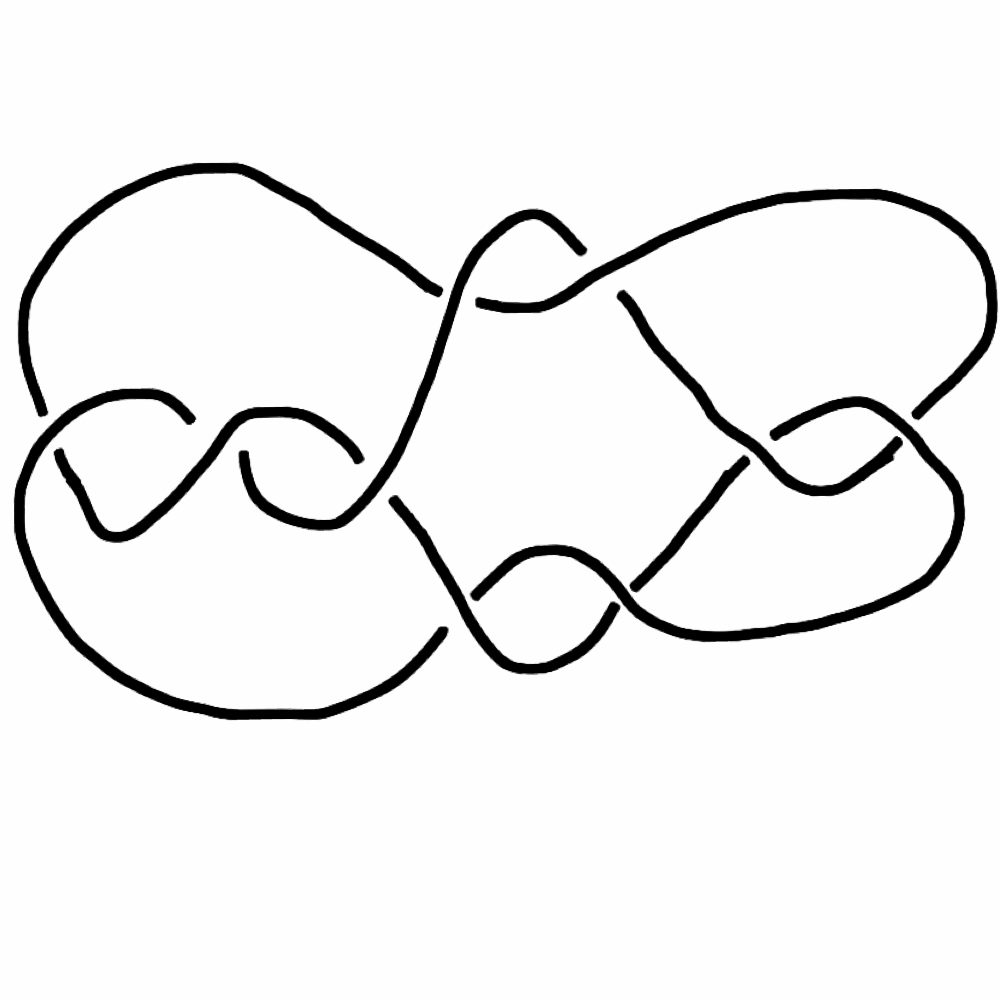
\includegraphics[width=.4\textwidth]{knotpics/goeritz.png}
    \caption{Goeritz's unknot}
\end{figure}

\begin{thebibliography}{9}

\bibitem{Adams}
    C.~Adams,
    \emph{The Knot Book: An elementary introduction to the mathematical theory of knots},
    W.~H.~Freeman Co., New York 1994.

\bibitem{AB}
    J.~W.~Alexander and G.~B.~Briggs,
    On types of knotted curves,
    Annals of Mathematics, 28 (1926/27) 562--586

\bibitem{G}
    L.~Goeritz, Bemerkungen zur knotentheorie,
    Abh. Math. Sem. Univ. Hamburg 10 (1934), 201--210.1

\bibitem{H-L}
    J.~Haas and J.~C.~Lagarias,
    The number of Reidemeister Moves Needed for Unknotting,
    Journal of the American Mathematical Society, 14 (2001), 399--428.

\bibitem{Haken}
    W. Haken,
    Theorie der Normalflachen, ein Iosotpie Kriterium f\"{u}r ein Kreis,
    Acta Mathematica, 105 (1961), 245--375.

\bibitem{R}
    H.~Reidemeister,
    Elementare Begr\"{u}ndang der Knotentheorie,
    Abh. Math. Sem. Univ. Hamburg, 5 (1926), 24--32.

%\bibitem{Demaine}
%    Erik Demaine, Martin Demaine, Yair Minsky, Joseph Mitchell, Ronald Rivest, \& Mihai Patrascu,
%    Picture Hanging Puzzles,
%    available online at the arXiv: 1203.3602v1,
%    16 March 2012

\end{thebibliography}

\end{document}
%sagemathcloud={"zoom_width":100}